%5_binomial_distribution.tex

%notes for the course Mathematics for Computer Scientists A
%taught at the University of Bristol
%2020_21 Conor Houghton conor.houghton@bristol.ac.uk

%To the extent possible under law, the author has dedicated all copyright 
%and related and neighboring rights to these notes to the public domain 
%worldwide. These notes are distributed without any warranty. 


\documentclass[11pt,a4paper]{scrartcl}
\typearea{12}
\usepackage{graphicx}
%\usepackage{pstricks}
\usepackage{listings}
\usepackage{color}


\newif\ifind
\indtrue


\lstset{language=C}
\usepackage{fancyhdr}
\pagestyle{fancy}
\usepackage{listings}
\usepackage{color}
\lstset{language=C}
\usepackage{fancyhdr}
\pagestyle{fancy}
\lfoot{\texttt{cs-uob.github.io/COMS10014/}}
\rfoot{\texttt{coms10011.github.com}}
\lhead{COMS10014 Binomial Distribution - Conor}
\begin{document}

\section*{5 The binomial distribution}

Say you roll a dice five times, what is the chance you get exactly
three sixes? There are three parts to working out the
probability. First consider the chance of getting three sixes in the
first three rolls. This is $(1/6)^3$. Next consider the change of
getting not-a-six in the next two rolls. This is $(5/6)^2$. Finally,
we are not just interested in getting three sixes followed by two
not-sixes: we want to count all the ways to get exactly three sixes
out of five rolls. This means we also need to count the number of ways
of choosing which three of the five rolls gives a six. Putting all
this together and using $R$ to denote the number of sixes
\begin{equation}
p(R=3)=\left(\begin{array}{c}5\\3\end{array}\right)\left(\frac{1}{6}\right)^3\left(\frac{5}{6}\right)^2=0.032
\end{equation}

This is an example of the \textbf{binomial distribution}; the binomial
distribution is important because it describes the result of multiple
independent trials. In a \textbf{binomial experiment}  
\begin{itemize}
\item There are $n$ identical trials.
\item Each trial has one of two outcomes, which we call success, $S$,
  and failure, $F$.
\item The trials are independent.
\item The random variable of interest, say $R$, is the total number of successes.
\end{itemize}
Lets call the chance of success for an individual trial $p$ and the
probability of failure $q=1-p$. By reasoning similar to that used in
the example above, it is easy to see
\begin{equation}
p_R(r)=\left(\begin{array}{c}n\\r\end{array}\right)p^rq^{n-r}
\end{equation}
Examples are plot in Fig.~\ref{fig_binomial}.

\begin{figure}[htb]
\begin{center}
% GNUPLOT: LaTeX picture with Postscript
\begingroup
  \makeatletter
  \providecommand\color[2][]{%
    \GenericError{(gnuplot) \space\space\space\@spaces}{%
      Package color not loaded in conjunction with
      terminal option `colourtext'%
    }{See the gnuplot documentation for explanation.%
    }{Either use 'blacktext' in gnuplot or load the package
      color.sty in LaTeX.}%
    \renewcommand\color[2][]{}%
  }%
  \providecommand\includegraphics[2][]{%
    \GenericError{(gnuplot) \space\space\space\@spaces}{%
      Package graphicx or graphics not loaded%
    }{See the gnuplot documentation for explanation.%
    }{The gnuplot epslatex terminal needs graphicx.sty or graphics.sty.}%
    \renewcommand\includegraphics[2][]{}%
  }%
  \providecommand\rotatebox[2]{#2}%
  \@ifundefined{ifGPcolor}{%
    \newif\ifGPcolor
    \GPcolorfalse
  }{}%
  \@ifundefined{ifGPblacktext}{%
    \newif\ifGPblacktext
    \GPblacktexttrue
  }{}%
  % define a \g@addto@macro without @ in the name:
  \let\gplgaddtomacro\g@addto@macro
  % define empty templates for all commands taking text:
  \gdef\gplbacktext{}%
  \gdef\gplfronttext{}%
  \makeatother
  \ifGPblacktext
    % no textcolor at all
    \def\colorrgb#1{}%
    \def\colorgray#1{}%
  \else
    % gray or color?
    \ifGPcolor
      \def\colorrgb#1{\color[rgb]{#1}}%
      \def\colorgray#1{\color[gray]{#1}}%
      \expandafter\def\csname LTw\endcsname{\color{white}}%
      \expandafter\def\csname LTb\endcsname{\color{black}}%
      \expandafter\def\csname LTa\endcsname{\color{black}}%
      \expandafter\def\csname LT0\endcsname{\color[rgb]{1,0,0}}%
      \expandafter\def\csname LT1\endcsname{\color[rgb]{0,1,0}}%
      \expandafter\def\csname LT2\endcsname{\color[rgb]{0,0,1}}%
      \expandafter\def\csname LT3\endcsname{\color[rgb]{1,0,1}}%
      \expandafter\def\csname LT4\endcsname{\color[rgb]{0,1,1}}%
      \expandafter\def\csname LT5\endcsname{\color[rgb]{1,1,0}}%
      \expandafter\def\csname LT6\endcsname{\color[rgb]{0,0,0}}%
      \expandafter\def\csname LT7\endcsname{\color[rgb]{1,0.3,0}}%
      \expandafter\def\csname LT8\endcsname{\color[rgb]{0.5,0.5,0.5}}%
    \else
      % gray
      \def\colorrgb#1{\color{black}}%
      \def\colorgray#1{\color[gray]{#1}}%
      \expandafter\def\csname LTw\endcsname{\color{white}}%
      \expandafter\def\csname LTb\endcsname{\color{black}}%
      \expandafter\def\csname LTa\endcsname{\color{black}}%
      \expandafter\def\csname LT0\endcsname{\color{black}}%
      \expandafter\def\csname LT1\endcsname{\color{black}}%
      \expandafter\def\csname LT2\endcsname{\color{black}}%
      \expandafter\def\csname LT3\endcsname{\color{black}}%
      \expandafter\def\csname LT4\endcsname{\color{black}}%
      \expandafter\def\csname LT5\endcsname{\color{black}}%
      \expandafter\def\csname LT6\endcsname{\color{black}}%
      \expandafter\def\csname LT7\endcsname{\color{black}}%
      \expandafter\def\csname LT8\endcsname{\color{black}}%
    \fi
  \fi
  \setlength{\unitlength}{0.0500bp}%
  \begin{picture}(5040.00,3528.00)%
    \gplgaddtomacro\gplbacktext{%
      \csname LTb\endcsname%
      \put(990,440){\makebox(0,0)[r]{\strut{} 0}}%
      \put(990,865){\makebox(0,0)[r]{\strut{} 0.025}}%
      \put(990,1289){\makebox(0,0)[r]{\strut{} 0.05}}%
      \put(990,1714){\makebox(0,0)[r]{\strut{} 0.075}}%
      \put(990,2138){\makebox(0,0)[r]{\strut{} 0.1}}%
      \put(990,2563){\makebox(0,0)[r]{\strut{} 0.125}}%
      \put(990,2987){\makebox(0,0)[r]{\strut{} 0.15}}%
      \put(1122,220){\makebox(0,0){\strut{}-5}}%
      \put(1562,220){\makebox(0,0){\strut{} 0}}%
      \put(2002,220){\makebox(0,0){\strut{} 5}}%
      \put(2442,220){\makebox(0,0){\strut{} 10}}%
      \put(2883,220){\makebox(0,0){\strut{} 15}}%
      \put(3323,220){\makebox(0,0){\strut{} 20}}%
      \put(3763,220){\makebox(0,0){\strut{} 25}}%
      \put(4203,220){\makebox(0,0){\strut{} 30}}%
      \put(4643,220){\makebox(0,0){\strut{} 35}}%
    }%
    \gplgaddtomacro\gplfronttext{%
      \csname LTb\endcsname%
      \put(3656,3090){\makebox(0,0)[r]{\strut{}$p$=0.25}}%
      \csname LTb\endcsname%
      \put(3656,2870){\makebox(0,0)[r]{\strut{}$p$=0.5}}%
    }%
    \gplbacktext
    \put(0,0){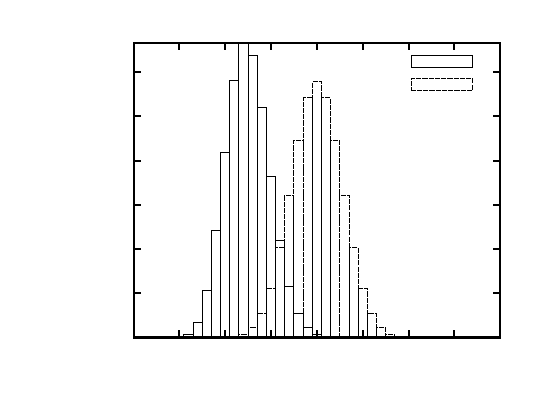
\includegraphics{binomial}}%
    \gplfronttext
  \end{picture}%
\endgroup

\end{center}
\caption{Binomial histograms. Here the value of $p_R(r)$ is plotted where $R$ is a binomial with $n=30$. In the left distribution $p=0.25$ and in the right $p=0.5$.\label{fig_binomial}}
\end{figure}

Say a student is doing a multiple choice vocabulary test in a language
that is very different from the one they speak or any they have never
learned, so they guess all the questions. If there are four options
for each question and fifteen questions, lets calculate $p(5)$, the
chance they get five correct:
\begin{equation}
p(R=5)=\left(\begin{array}{c}15\\5\end{array}\right)(0.25)^5(0.75)^{10}=0.165
\end{equation}

Hopefully you will have seen the binomial coefficient before in the
expansion of polynomials:
\begin{equation}
(q+p)^n=q^n+nq^{n-1}p+\left(\begin{array}{c}n\\2\end{array}\right)q^{n-2}p^2+\ldots+p^n=\sum_{r=0}^n \left(\begin{array}{c}n\\r\end{array}\right)p^rq^{n-r}
\end{equation}
Applied to our case, where $q=1-p$, the left hand side is one; the right hand side is a sum over the probabilities.
\begin{equation}
1=\sum_{r=0}^n \left(\begin{array}{c}n\\r\end{array}\right)p^rq^{n-r}=\sum_{r=0}^np(R=r)
\end{equation}
This is what you would expect, the probabilities should add to
one. However, this formula leads to a very neat trick, first:
\begin{equation}
1=\sum_{r=0}^n \left(\begin{array}{c}n\\r\end{array}\right)p^rq^{n-r}
\end{equation}
Now differentiate both sides with $p$, so take $d/dp$. The left side is a constant so it differentiates to zero and we have
\begin{equation}
0=\sum_{r=0}^n
\left(\begin{array}{c}n\\r\end{array}\right)rp^{r-1}q^{n-r}-\sum_{r=0}^n
  \left(\begin{array}{c}n\\r\end{array}\right)p^r(n-r)q^{n-r-1}
\end{equation}
where we have used the product rule, remembering that $q=1-p$. Next we multiply and divide by either $p$ or $q$, it will be clear why in a few lines time:
\begin{equation}
0=\frac{1}{p}\sum_{r=0}^n \left(\begin{array}{c}n\\r\end{array}\right)rp^rq^{n-r}
-\frac{1}{q}\sum_{r=0}^n \left(\begin{array}{c}n\\r\end{array}\right)p^r(n-r)q^{n-r}
\end{equation}
Now, $n$ is just a constant so we can go
\begin{equation}
\sum_{r=0}^n \left(\begin{array}{c}n\\r\end{array}\right)np^rq^{n-r}=n\sum_{r=0}^n \left(\begin{array}{c}n\\r\end{array}\right)p^rq^{n-r}=n
\end{equation}
Once we deal with this part we see we have two terms that look the same except for the $1/p$ or $1/q$ at the start, 
\begin{equation}
0=\frac{n}{q}-\left(\frac{1}{q}+\frac{1}{p}\right)\sum_{r=0}^n \left(\begin{array}{c}n\\r\end{array}\right)p^rrq^{n-r}
\end{equation}
However, be definition
\begin{equation}
\langle R\rangle=\sum_{r=0}^n p(R=r)r=\sum_{r=0}^n \left(\begin{array}{c}n\\r\end{array}\right)p^rrq^{n-r}
\end{equation}
so
\begin{equation}
\left(\frac{1}{p}+\frac{1}{q}\right)\langle R\rangle=\frac{n}{q}
\end{equation}
It only remains to note
\begin{equation}
\frac{1}{p}+\frac{1}{q}=\frac{q+p}{pq}=\frac{1}{pq}
\end{equation}
to derive
\begin{equation}
\langle R\rangle=pn
\end{equation}

A similar argument based on differentiating twice gives the standard
deviation:
\begin{equation}
\sigma^2=pqn
\end{equation}

\ifind
\section*{Summary}
\else
\subsection*{9 Gauss distribution}
\fi

\begin{itemize}

\item The \textbf{Gau\ss{}ian distribution} has density
  \begin{equation}
p(x)=\frac{1}{\sqrt{2\pi\sigma^2}}e^{-\frac{(x-\mu)^2}{2\sigma^2}}
  \end{equation}


\item You can  shown that the mean is $\mu$ and the variance is $\sigma^2$ as the notation would suggest by differenciating
\begin{equation}
1=Z=\int_{-\infty}^\infty p(x)dx
\end{equation}
with respect to $\mu$.

%\item It has moment generating function
%  \begin{equation}
%m(t)= e^{\mu t + \frac{1}{2}\sigma^2 t^2}
%  \end{equation}
%  from which can be be shown that the mean is $\mu$ and the variance is $\sigma%^2$ as the notation would suggest.

\item To work out probabilities you need to use the \textbf{error function}
  \begin{equation}
\mbox{erf}\,(x)=\frac{1}{\sqrt{\pi}}\int_{-x}^xe^{-y^2}dy=\frac{2}{\sqrt{\pi}}\int_0^xe^{-y^2}dy
  \end{equation}
  In fact
  \begin{equation}
\mbox{Prob}(x_1<x<x_2)=\frac{1}{2}[\mbox{erf}\,(z_2)-\mbox{erf}\,(z_1)]
  \end{equation}
  where
  \begin{equation}
z=\frac{x-\mu}{\sqrt{2}\sigma}
  \end{equation}
  \end{itemize}


\ifind
\section*{Example question}
\else
\subsection*{2 conditional probability - example question}
\fi

This is known as the `second sibling' problem and like the Monty Hall problem it was popularized by Marilyn Vos Savant:
\begin{quote}
 A shopkeeper says she has two new baby beagles to show you, but
    she doesn't know whether they're male, female, or a pair. You tell
    her that you want only a male, and she telephones the fellow who's
    giving them a bath. "Is at least one a male?" she asks him. "Yes!"
    she informs you with a smile. What is the probability that the
    other one is a male?
\end{quote}

\noindent \textbf{solution} So we are assuming that males and females are equally likely and that the sex of the two pups is independent; the set of outcomes, using the obvious notation, is $\mathcal{X}=\{(m,m),(m,f),(f,m),(f,f)\}$ with each event having probability $1/4$. The event that at least one is male is $\mathcal{M}=\{(m,m),(m,f),(f,m)\}$. This means that $P(\mathcal{M})=3/4$. Lets call the event that the second dog is male $\mathcal{S}$ so $\mathcal{M}\cap\mathcal{S}=\{(m,m)\}$ and
\begin{equation}
P(\mathcal{M}\cap\mathcal{S})=\frac{1}{4}
\end{equation}
and hence
\begin{equation}
P(\mathcal{S}|\mathcal{M})=\frac{1}{3}
\end{equation}
and so the probability the second dog is male is one in three.



\end{document}




